\renewcommand{\thesubsubsection}{\alph{subsubsection})}
\setcounter{section}{2}
\setcounter{subsection}{0}

\subsection{Short project info (5pts)}

\subsection{Optimization blockers (30pts)}
\subsubsection{} % a)
\autoref{fig:1a} shows the plot of the runtime in cycles of the various implementations of the original function. These benchmarks were performed on an \textit{Intel Xeon Silver 4210 @ 2.20 GHz Cascade Lake} and the code was compiled using \textit{GCC 11.2.1} with flags \texttt{-O3}, \texttt{-march=skylake}, \texttt{-mno-fma} and \texttt{-fno-tree-vectorize}.
\begin{table}[h!]
    \centering
    \begin{tabular}{l|llll}
    \hline
    Implementation & Baseline & V1 & V2 & V3 \\
    Runtime (cycles) & \input{../out/ex2_a_baseline.txt} & \input{../out/ex2_a_v1.txt} & \input{../out/ex2_a_v2.txt} & \input{../out/ex2_a_v3.txt}\\
    \hline
    \end{tabular}
    \caption{Comparison of the function implementations}
    \vspace*{-0.3cm}
\end{table}

\textbf{Baseline}\\
The original provided baseline implementation. It is the slowest of all the implementations.

\textbf{V1}
\vspace*{-0.3cm}
\begin{enumerate}
\item Uses $2x$ loop unrolling on the outer loop, $6x$ for the inner loop, and $4x$ for the final loop. 
\item All function invocations are removed, and replaced with direct access to the \texttt{data} matrix. 
\item This implementation also makes use of the assumption that $n=100$ for every square $n*n$ matrix, therefore it uses the numeric constant 100 for the matrix bound check. 
\end{enumerate}
We notice how removing the function invocation overhead and adding loop unrolling already provides a significant speedup of almost $2x$ over the baseline.

\textbf{V2}
\vspace*{-0.3cm}
\begin{enumerate}
    \item In this implementation we simplify the data fetching that uses the modulo operator. Since we are performing $6x$ loop unrolling, we can simplify the modulo 3 and modulo 6 expressions by replacing them with constant values in the range $[0, 5]$. 
    \item Simplified the \texttt{abs(fmax(...))+1} statements in the last loop with the ternary operator.
    \item Introduced precomputation of all independent \texttt{sqrt} statements outside of the loop body.
    \item Each division by a \texttt{sqrt} is replaced with a multiplication by the inverse of the \texttt{sqrt} value, also precomputed. This was done to avoid costly divisions in the loop body.
\end{enumerate}

\textbf{V3}
\vspace*{-0.3cm}
\begin{enumerate}
\item In this last version we exploit the periodicity of the cosine function to precompute the values of the \texttt{cos} function outside of the loop body.
\item Analogously to the previous version, we also precompute the reciprocal of the \texttt{cos} values to avoid costly divisions in the loop body.
\item We also merge the ternary operations of the last loop into the first loop.
\end{enumerate}
We notice how precomputing the cosine values yields by far the biggest performance improvement. The last implementation is clearly the fastest, yielding a speedup of \textbf{\input{../out/ex2_cspeedup.txt}} over the baseline.
\begin{figure}[h!]
    \centering
    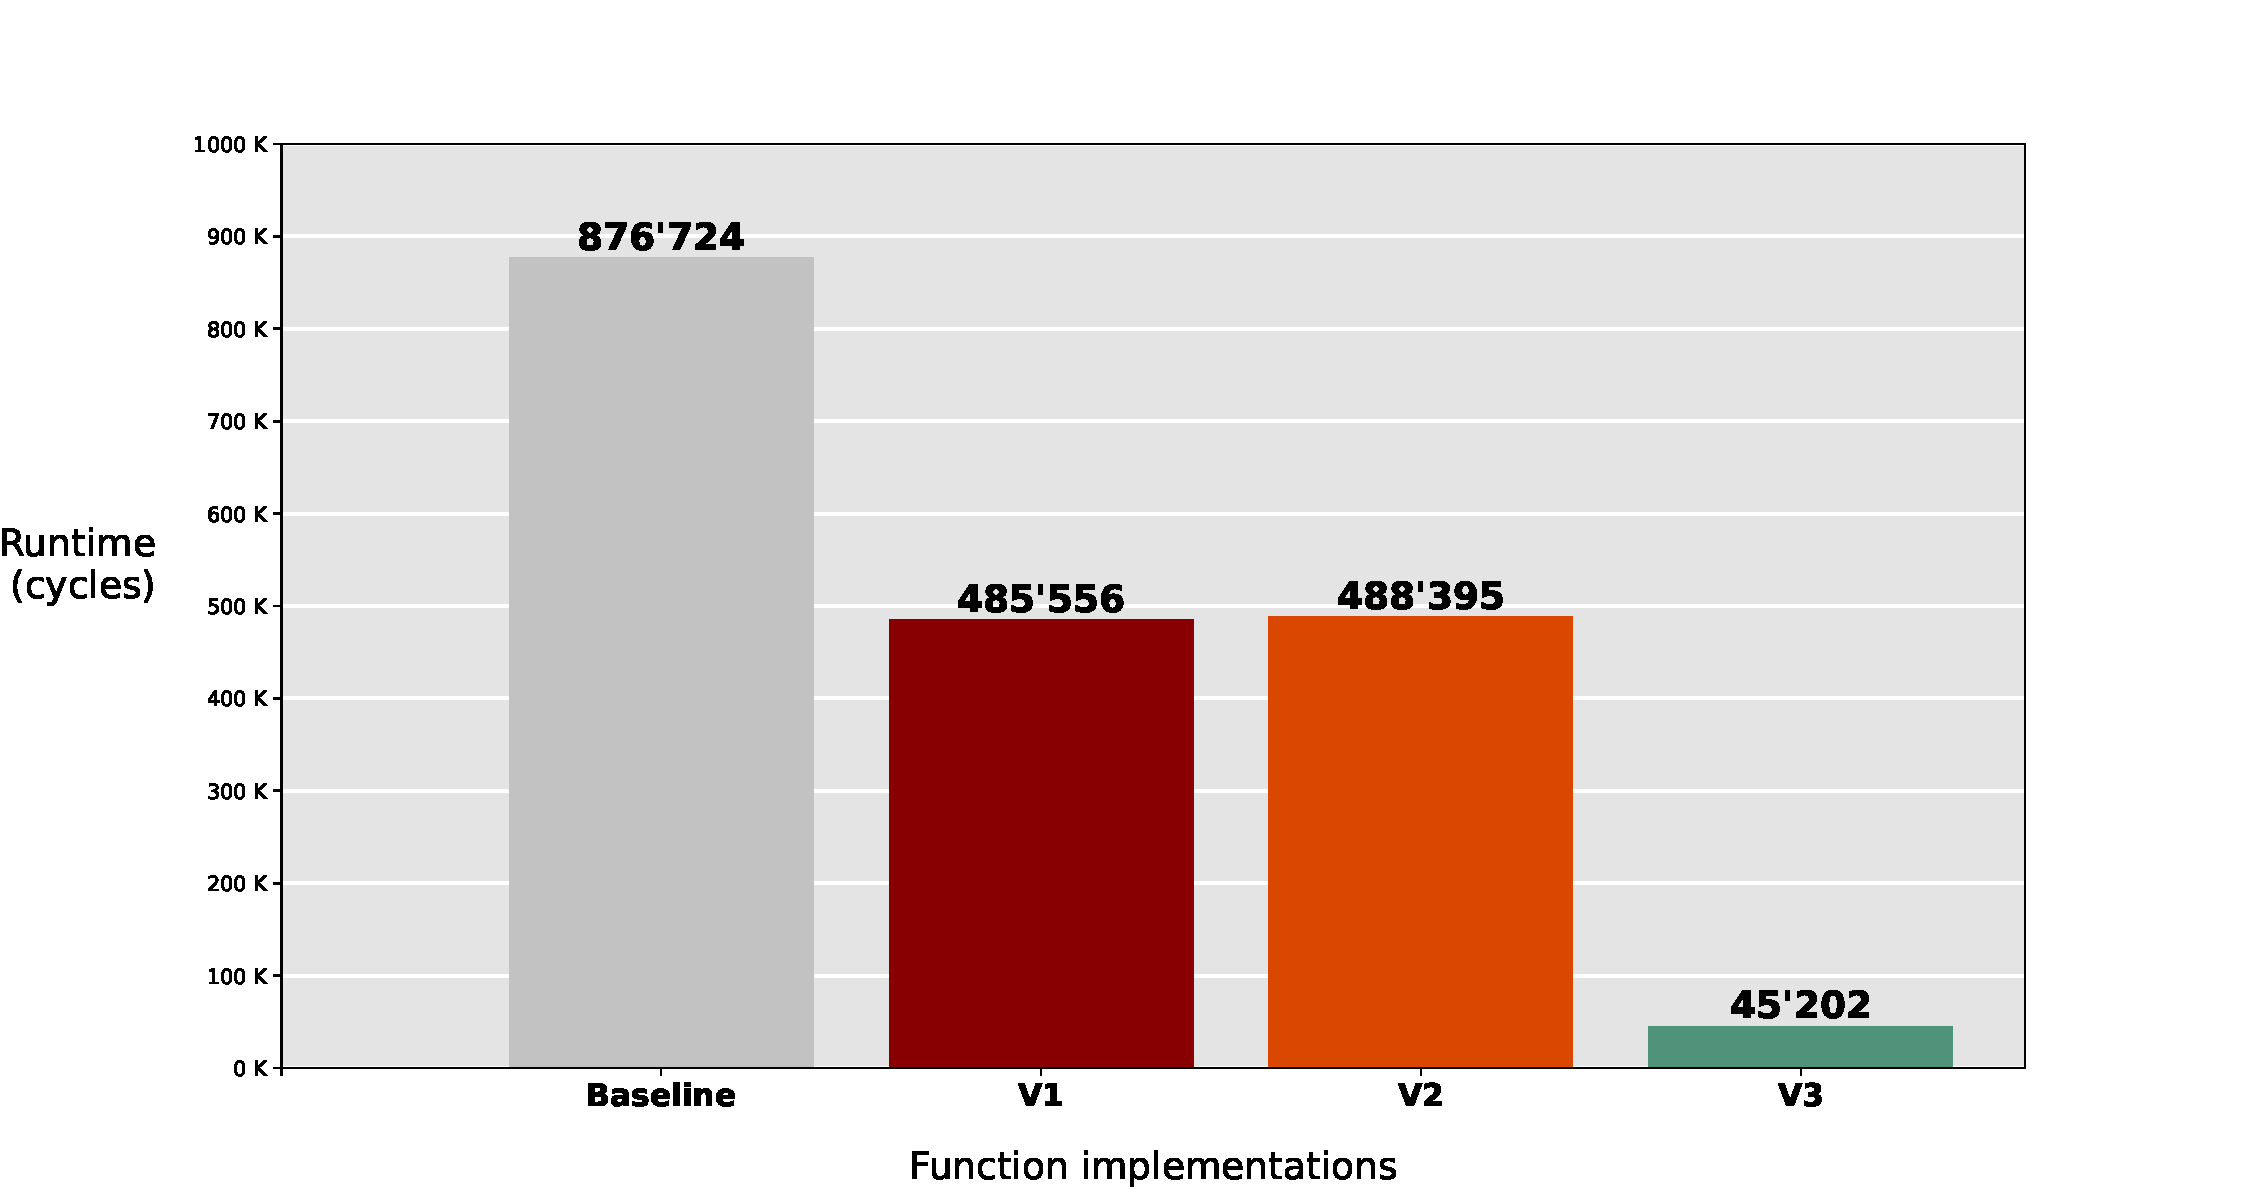
\includegraphics[width=\linewidth]{../out/ex2_a.pdf}
    \caption{Runtime comparison of the function implementations}
    \label{fig:1a}
\end{figure}

\subsubsection{} % b)
The \texttt{V3} implementation performs 50 iterations in outer loop and 16 in the inner loop, therefore $W =\input{../out/ex2_b_flopsformula.txt} = \input{../out/ex2_b_flops.txt}$ flops. The performance is therefore $\pi = \frac{\input{../out/ex2_b_flops.txt}}{\input{../out/ex2_a_v3.txt}} = \input{../out/ex2_b.txt}$ flops/cycle.
\subsubsection{} % c)
The theoretical peak performance is 2 flops/cycles. The performance of the \texttt{V3} implementation is $\input{../out/ex2_b.txt}$ flops/cycle, which is $\input{../out/ex2_c.txt}$\% of the theoretical peak performance.

\subsection{Microbenchmarks (40 pts)}
\subsubsection{} % a)

\subsubsection{} % b)

\subsubsection{} % c)
